%! Author = Omar Iskandarani
%! Title = Appendix: Experimental Validation of the Vortex-Core Tangential Velocity $C_e$
%! Date = June 17, 2025
%! Affiliation = Independent Researcher, Groningen, The Netherlands
%! License = CC-BY 4.0
%! ORCID = 0009-0006-1686-3961
%! DOI = 10.5281/zenodo.15692509

% === Metadata ===
%\newcommand{\appendixtitle}{\textbf{Experimental Proposal: Gravitational Modulation via Resonant Vortex Structures in Æther}}
%\newcommand{\paperdoi}{10.5281/zenodo.15692509}
%
%
%\ifdefined\standalonechapter\else
%% Standalone mode
%\documentclass[12pt]{article}
%\usepackage{tcolorbox}
%% vamstyle.sty
\NeedsTeXFormat{LaTeX2e}
\ProvidesPackage{vamstyle}[2025/07/01 VAM unified style]

% === Constants ===
\newcommand{\hbarVal}{\ensuremath{1.054571817 \times 10^{-34}}} % J\cdot s
\newcommand{\meVal}{\ensuremath{9.10938356 \times 10^{-31}}} % kg
\newcommand{\cVal}{\ensuremath{2.99792458 \times 10^{8}}} % m/s
\newcommand{\alphaVal}{\ensuremath{1 / 137.035999084}} % unitless
\newcommand{\alphaGVal}{\ensuremath{1.75180000 \times 10^{-45}}} % unitless
\newcommand{\reVal}{\ensuremath{2.8179403227 \times 10^{-15}}} % m
\newcommand{\rcVal}{\ensuremath{1.40897017 \times 10^{-15}}} % m
\newcommand{\vacrho}{\ensuremath{5 \times 10^{-9}}} % kg/m^3
\newcommand{\LpVal}{\ensuremath{1.61625500 \times 10^{-35}}} % m
\newcommand{\MpVal}{\ensuremath{2.17643400 \times 10^{-8}}} % kg
\newcommand{\tpVal}{\ensuremath{5.39124700 \times 10^{-44}}} % s
\newcommand{\TpVal}{\ensuremath{1.41678400 \times 10^{32}}} % K
\newcommand{\qpVal}{\ensuremath{1.87554596 \times 10^{-18}}} % C
\newcommand{\EpVal}{\ensuremath{1.95600000 \times 10^{9}}} % J
\newcommand{\eVal}{\ensuremath{1.60217663 \times 10^{-19}}} % C

% === VAM/\ae ther Specific ===
\newcommand{\CeVal}{\ensuremath{1.09384563 \times 10^{6}}} % m/s
\newcommand{\FmaxVal}{\ensuremath{29.0535070}} % N
\newcommand{\FmaxGRVal}{\ensuremath{3.02563891 \times 10^{43}}} % N
\newcommand{\gammaVal}{\ensuremath{0.005901}} % unitless
\newcommand{\GVal}{\ensuremath{6.67430000 \times 10^{-11}}} % m^3/kg/s^2
\newcommand{\hVal}{\ensuremath{6.62607015 \times 10^{-34}}} % J Hz^-1

% === Electromagnetic ===
\newcommand{\muZeroVal}{\ensuremath{1.25663706 \times 10^{-6}}}
\newcommand{\epsilonZeroVal}{\ensuremath{8.85418782 \times 10^{-12}}}
\newcommand{\ZzeroVal}{\ensuremath{3.76730313 \times 10^{2}}}

% === Atomic & Thermodynamic ===
\newcommand{\RinfVal}{\ensuremath{1.09737316 \times 10^{7}}}
\newcommand{\aZeroVal}{\ensuremath{5.29177211 \times 10^{-11}}}
\newcommand{\MeVal}{\ensuremath{9.10938370 \times 10^{-31}}}
\newcommand{\MprotonVal}{\ensuremath{1.67262192 \times 10^{-27}}}
\newcommand{\MneutronVal}{\ensuremath{1.67492750 \times 10^{-27}}}
\newcommand{\kBVal}{\ensuremath{1.38064900 \times 10^{-23}}}
\newcommand{\RVal}{\ensuremath{8.31446262}}

% === Compton, Quantum, Radiation ===
\newcommand{\fCVal}{\ensuremath{1.23558996 \times 10^{20}}}
\newcommand{\OmegaCVal}{\ensuremath{7.76344071 \times 10^{20}}}
\newcommand{\lambdaCVal}{\ensuremath{2.42631024 \times 10^{-12}}}
\newcommand{\PhiZeroVal}{\ensuremath{2.06783385 \times 10^{-15}}}
\newcommand{\phiVal}{\ensuremath{1.61803399}}
\newcommand{\eVVal}{\ensuremath{1.60217663 \times 10^{-19}}}
\newcommand{\GFVal}{\ensuremath{1.16637870 \times 10^{-5}}}
\newcommand{\lambdaProtonVal}{\ensuremath{1.32140986 \times 10^{-15}}}
\newcommand{\ERinfVal}{\ensuremath{2.17987236 \times 10^{-18}}}
\newcommand{\fRinfVal}{\ensuremath{3.28984196 \times 10^{15}}}
\newcommand{\sigmaSBVal}{\ensuremath{5.67037442 \times 10^{-8}}}
\newcommand{\WienVal}{\ensuremath{2.89777196 \times 10^{-3}}}
\newcommand{\kEVal}{\ensuremath{8.98755179 \times 10^{9}}}

% === \ae ther Densities ===
\newcommand{\rhoMass}{\rho_\text{\ae}^{(\text{mass})}}
\newcommand{\rhoMassVal}{\ensuremath{3.89343583 \times 10^{18}}}
\newcommand{\rhoEnergy}{\rho_\text{\ae}^{(\text{energy})}}
\newcommand{\rhoEnergyVal}{\ensuremath{3.49924562 \times 10^{35}}}
\newcommand{\rhoFluid}{\rho_\text{\ae}^{(\text{fluid})}}
\newcommand{\rhoFluidVal}{\ensuremath{7.00000000 \times 10^{-7}}}

% === Draft Options ===
\newif\ifvamdraft
% \vamdrafttrue
\ifvamdraft
\RequirePackage{showframe}
\fi

% === Load Once ===
\RequirePackage{ifthen}
\newboolean{vamstyleloaded}
\ifthenelse{\boolean{vamstyleloaded}}{}{\setboolean{vamstyleloaded}{true}

% === Page ===
\RequirePackage[a4paper, margin=2.5cm]{geometry}

% === Fonts ===
\RequirePackage[T1]{fontenc}
\RequirePackage[utf8]{inputenc}
\RequirePackage[english]{babel}
\RequirePackage{textgreek}
\RequirePackage{mathpazo}
\RequirePackage[scaled=0.95]{inconsolata}
\RequirePackage{helvet}

% === Math ===
\RequirePackage{amsmath, amssymb, mathrsfs, physics}
\RequirePackage{siunitx}
\sisetup{per-mode=symbol}

% === Tables ===
\RequirePackage{graphicx, float, booktabs}
\RequirePackage{array, tabularx, multirow, makecell}
\newcolumntype{Y}{>{\centering\arraybackslash}X}
\newenvironment{tighttable}[1][]{\begin{table}[H]\centering\renewcommand{\arraystretch}{1.3}\begin{tabularx}{\textwidth}{#1}}{\end{tabularx}\end{table}}
\RequirePackage{etoolbox}
\newcommand{\fitbox}[2][\linewidth]{\makebox[#1]{\resizebox{#1}{!}{#2}}}

% === Graphics ===
\RequirePackage{tikz}
\usetikzlibrary{3d, calc, arrows.meta, positioning}
\RequirePackage{pgfplots}
\pgfplotsset{compat=1.18}
\RequirePackage{xcolor}

% === Code ===
\RequirePackage{listings}
\lstset{basicstyle=\ttfamily\footnotesize, breaklines=true}

% === Theorems ===
\newtheorem{theorem}{Theorem}[section]
\newtheorem{lemma}[theorem]{Lemma}

% === TOC ===
\RequirePackage{tocloft}
\setcounter{tocdepth}{2}
\renewcommand{\cftsecfont}{\bfseries}
\renewcommand{\cftsubsecfont}{\itshape}
\renewcommand{\cftsecleader}{\cftdotfill{.}}
\renewcommand{\contentsname}{\centering \Huge\textbf{Contents}}

% === Sections ===
\RequirePackage{sectsty}
\sectionfont{\Large\bfseries\sffamily}
\subsectionfont{\large\bfseries\sffamily}

% === Bibliography ===
\RequirePackage[numbers]{natbib}

% === Links ===
\RequirePackage{hyperref}
\hypersetup{
    colorlinks=true,
    linkcolor=blue,
    citecolor=blue,
    urlcolor=blue,
    pdftitle={The Vortex \AE ther Model},
    pdfauthor={Omar Iskandarani},
    pdfkeywords={vorticity, gravity, \ae ther, fluid dynamics, time dilation, VAM}
}
\urlstyle{same}
\RequirePackage{bookmark}

% === Misc ===
\RequirePackage[none]{hyphenat}
\sloppy
\RequirePackage{empheq}
\RequirePackage[most]{tcolorbox}
\newtcolorbox{eqbox}{colback=blue!5!white, colframe=blue!75!black, boxrule=0.6pt, arc=4pt, left=6pt, right=6pt, top=4pt, bottom=4pt}
\RequirePackage{titling}
\RequirePackage{amsfonts}
\RequirePackage{titlesec}
\RequirePackage{enumitem}

\AtBeginDocument{\RenewCommandCopy\qty\SI}

\pretitle{\begin{center}\LARGE\bfseries}
\posttitle{\par\end{center}\vskip 0.5em}
\preauthor{\begin{center}\large}
\postauthor{\end{center}}
\predate{\begin{center}\small}
\postdate{\end{center}}

\endinput
}
%% vamappendixsetup.sty

\newcommand{\titlepageOpen}{
  \begin{titlepage}
  \thispagestyle{empty}
  \centering
  {\Huge\bfseries \papertitle \par}
  \vspace{1cm}
  {\Large\itshape\textbf{Omar Iskandarani}\textsuperscript{\textbf{*}} \par}
  \vspace{0.5cm}
  {\large \today \par}
  \vspace{0.5cm}
}

% here comes abstract
\newcommand{\titlepageClose}{
  \vfill
  \null
  \begin{picture}(0,0)
  % Adjust position: (x,y) = (left, bottom)
  \put(-200,-40){  % Shift 75pt left, 40pt down
    \begin{minipage}[b]{0.7\textwidth}
    \footnotesize % One step bigger than \tiny
    \renewcommand{\arraystretch}{1.0}
    \noindent\rule{\textwidth}{0.4pt} \\[0.5em]  % ← horizontal line
    \textsuperscript{\textbf{*}}Independent Researcher, Groningen, The Netherlands \\
    Email: \texttt{info@omariskandarani.com} \\
    ORCID: \texttt{\href{https://orcid.org/0009-0006-1686-3961}{0009-0006-1686-3961}} \\
    DOI: \href{https://doi.org/\paperdoi}{\paperdoi} \\
    License: CC-BY 4.0 International \\
    \end{minipage}
  }
  \end{picture}
  \end{titlepage}
}
%\begin{document}
%
%    % === Title page ===
%    \titlepageOpen
%
%    \begin{abstract}
%        We propose a falsifiable laboratory experiment to test whether gravitational effects can be modulated through controlled resonance in vortex-supporting materials, based on the Vortex \AE{}ther Model (VAM)~\cite{iskandarani2025vam2, iskandarani2025benchmark}. In contrast to general relativity, which treats gravity as spacetime curvature, VAM postulates that gravitation emerges from the angular momentum density of knotted vorticity fields embedded in an incompressible, inviscid superfluid \ae ther~\cite{iskandarani2025timedilation}. By engineering a system that dynamically modulates the swirl tangential velocity via the resonant condition \( C_e = f \cdot \Delta x \), we aim to generate a measurable change in the local gravitational potential.
%
%        The predicted gravitational acceleration shift is derived from the swirl-induced potential \(\Phi(r) \sim C_e^3\), where both frequency \(f\) and displacement amplitude \(\Delta x\) are externally tunable. Using thin-film SAW or FBAR resonators fabricated on piezoelectric substrates, and selecting vortex-active metals such as Pd, Au, or Ti, we create localized standing wave fields that simulate rotating vortex structures. Predicted changes in acceleration lie in the range \(10^{-10}\) to \(10^{-8} \, \text{m/s}^2\), within detection limits of state-of-the-art quantum gravimeters~\cite{iskandarani2025experimentalCe}.
%
%        This approach offers an experimentally accessible method to probe gravitational emergence via internal æther dynamics, extending the analogue gravity paradigm into a falsifiable physical test regime.
%    \end{abstract}
%
%
%    \titlepageClose
%    \fi
%
%    \ifdefined\standalonechapter
%    \section{\appendixtitle}
%    \else
%    \fi
% ============= Begin of content ============
    \section{\textbf{Experimental Proposal: Gravitational Modulation via Resonant Vortex Structures in Æther}}
    \section*{Abstract}
        We propose a falsifiable laboratory experiment to test whether gravitational effects can be modulated through controlled resonance in vortex-supporting materials, based on the Vortex \AE{}ther Model (VAM)~\cite{iskandarani2025vam2, iskandarani2025benchmark}. In contrast to general relativity, which treats gravity as spacetime curvature, VAM postulates that gravitation emerges from the angular momentum density of knotted vorticity fields embedded in an incompressible, inviscid superfluid \ae ther~\cite{iskandarani2025timedilation}. By engineering a system that dynamically modulates the swirl tangential velocity via the resonant condition \( C_e = f \cdot \Delta x \), we aim to generate a measurable change in the local gravitational potential.

        The predicted gravitational acceleration shift is derived from the swirl-induced potential \(\Phi(r) \sim C_e^3\), where both frequency \(f\) and displacement amplitude \(\Delta x\) are externally tunable. Using thin-film SAW or FBAR resonators fabricated on piezoelectric substrates, and selecting vortex-active metals such as Pd, Au, or Ti, we create localized standing wave fields that simulate rotating vortex structures. Predicted changes in acceleration lie in the range \(10^{-10}\) to \(10^{-8} \, \text{m/s}^2\), within detection limits of state-of-the-art quantum gravimeters~\cite{iskandarani2025experimentalCe}.

        This approach offers an experimentally accessible method to probe gravitational emergence via internal æther dynamics, extending the analogue gravity paradigm into a falsifiable physical test regime.


    \section*{Physical Motivation}
    In VAM, the gravitational potential associated with a localized vortex knot is:
    \begin{equation}
        \Phi(r) = \frac{C_e^3}{2 F_{\text{max}} r_c} \cdot r e^{-r / r_c}
    \end{equation}
    where:
    \begin{itemize}
        \item \( C_e = f \cdot \Delta x \): swirl tangential velocity
        \item \( F_{\text{max}} \): maximum ætheric force
        \item \( r_c \): vortex core radius
    \end{itemize}

    Changes in frequency \( f \) or amplitude \( \Delta x \) thus induce nonlinear changes in \( \Phi \), offering a pathway to direct gravitational modulation.

    \section*{Experimental Design}
    \subsection*{Apparatus}
    \begin{itemize}
        \item \textbf{Piezoelectric substrate:} Quartz, LiNbO$_3$, or AlN
        \item \textbf{Thin film layer:} Pd, Au, or Ti (vortex-active materials)
        \item \textbf{SAW/FBAR resonator:} Excite at \SI{10}{MHz}--\SI{200}{MHz}
        \item \textbf{Interferometric or gravimetric sensor:} Beneath active region
    \end{itemize}

    \subsection*{Procedure}
    \begin{enumerate}
        \item Deposit thin metal film onto piezoelectric wafer.
        \item Pattern IDTs (interdigital transducers) for SAW excitation.
        \item Modulate \( f \in [10, 200] \) MHz and \( \Delta x \in [10, 100] \) nm.
        \item Measure local gravitational influence using torsion balance, cold-atom interferometry, or nanogravimeter.
    \end{enumerate}

    \section*{Theoretical Prediction}
    Given \( C_e = f \cdot \Delta x \), we estimate:
    \begin{equation}
        \Delta \Phi \sim \frac{C_e^3}{2 F_{\text{max}} r_c} \Rightarrow \Delta g = -\dv{\Phi}{r} \sim A e^{-r/r_c} \left(1 - \frac{r}{r_c}\right)
    \end{equation}

    For target resonance conditions (\( f \sim 1 \, \text{GHz}, \Delta x \sim 1 \, \mu\text{m} \)), we expect:
    \begin{itemize}
        \item \( C_e \approx 10^6 \, \text{m/s} \)
        \item \( \Delta g \sim 10^{-10} \text{ to } 10^{-8} \, \text{m/s}^2 \)
    \end{itemize}
    This is detectable using advanced torsion balances or quantum gravimeters.

    \begin{table}[h!]
        \centering
        \begin{tabular}{|c|c|c|}
            \hline
            \textbf{Symbol} & \textbf{Value} & \textbf{Unit} \\
            \hline
            \( C_e \) & \( 1.09384563 \times 10^6 \) & m/s \\
            \( F_{\text{max}} \) & 29.053507 & N \\
            \( r_c \) & \( 1.40897017 \times 10^{-15} \) & m \\
            \( \rho_\text{\ae} \) & \( 7.0 \times 10^{-7} \) & kg/m$^3$ \\
            \( t_p \) & \( 5.391247 \times 10^{-44} \) & s \\
            \( c \) & \( 2.99792458 \times 10^8 \) & m/s \\
            \hline
        \end{tabular}
        \caption{Constants used in all numerical estimates and plots.}
    \end{table}


    \section*{Expected Outcomes and Interpretation}
    \begin{itemize}
        \item A reproducible modulation of local weight or phase delay would strongly support the VAM framework.
        \item Absence of such modulation within predicted bounds would constrain or falsify the core vortex-gravity relation.
    \end{itemize}

    \section*{Rotating Superfluid Analogy and Modulation Rationale}

    Rotating superfluids—such as helium-II and Bose-Einstein condensates—form quantized vortex lattices, where angular momentum is discretized into coherent topological defects. These structures not only characterize the internal flow dynamics but also give rise to macroscopic inertial effects. In the field of analogue gravity, such systems have been employed to simulate event horizons, frame-dragging, and even metric curvature, through engineered velocity profiles and phase coherence \cite{barcelo2005analogue, volovik2003universe}.

    The Vortex \AE{}ther Model (VAM) generalizes this insight into a physical gravitational hypothesis. Rather than treating these effects as analogues, VAM proposes that gravity \emph{is} an emergent manifestation of swirl energy in an incompressible, inviscid superfluid \ae ther. Within this framework, the local gravitational potential due to a structured vortex field is approximated as:
    \[
        \Phi(r) \sim \frac{|\vec{\omega}(r)|^2}{2 F_{\text{max}}} \sim \frac{C_e^2}{2 F_{\text{max}}} e^{-2r/r_c}
    \]
    where \( \vec{\omega}(r) \) is the vorticity magnitude, \( C_e = f \cdot \Delta x \) is the controllable swirl tangential velocity, and \( r_c \) is the vortex core radius.

    The proposed experiment modulates \( C_e \) via surface acoustic waves (SAWs) in piezoelectric-vortex-active structures~\cite{iskandarani2025experimentalCe}. This approach aims to actively vary the local swirl energy and hence test whether gravitational modulation can be induced. Such an effect—if detected—would parallel the Meissner effect in superconductors, where external fields are excluded through intrinsic collective behavior. However, here the modulation arises mechanically rather than electromagnetically.

    For modulation amplitudes \( \Delta x \sim 1 \, \mu\text{m} \) and resonant frequencies \( f \sim 1\, \text{GHz} \), we estimate \( C_e \sim 10^6 \, \text{m/s} \), leading to predicted gravitational acceleration shifts:
    \[
        \Delta g \sim \frac{C_e^2}{F_{\text{max}} r_c} e^{-2r/r_c}
    \]
    For reasonable estimates of \( F_{\text{max}} \sim 10^{12} \, \text{N/kg} \) and \( r_c \sim 1 \, \text{mm} \), this yields \( \Delta g \sim 10^{-10} \) to \( 10^{-8} \, \text{m/s}^2 \), which is above the detection threshold of modern torsion balances and cold-atom gravimeters \cite{packard1998superfluid, zmeev2018masssensor}.

    Unlike purely analogue models, VAM makes a falsifiable physical claim~\cite{iskandarani2025benchmark}: that externally imposed swirl modulation can alter local gravitational behavior. Detecting such modulation would challenge current understanding and potentially bridge hydrodynamic and gravitational field theories.

    \section*{Error Analysis and Predictive Modeling}

    \subsection*{Predicted Acceleration and Uncertainty}
    We define the effective gravitational acceleration from the swirl-induced potential:
    \begin{equation}
        \Delta g(r) = -\dv{\Phi}{r} = -\frac{C_e^3}{2 F_{\text{max}} r_c^2} \left(1 - \frac{r}{r_c}\right) e^{-r/r_c}
    \end{equation}

    We evaluate \( \Delta g \) numerically for multiple \( C_e \) values corresponding to practical ranges of \( f \in [10, 1000]\,\text{MHz} \) and \( \Delta x \in [10, 500]\,\text{nm} \).

    \subsection*{Simulation Plots of Potential and Acceleration}

    \begin{figure}[h!]
        \centering
        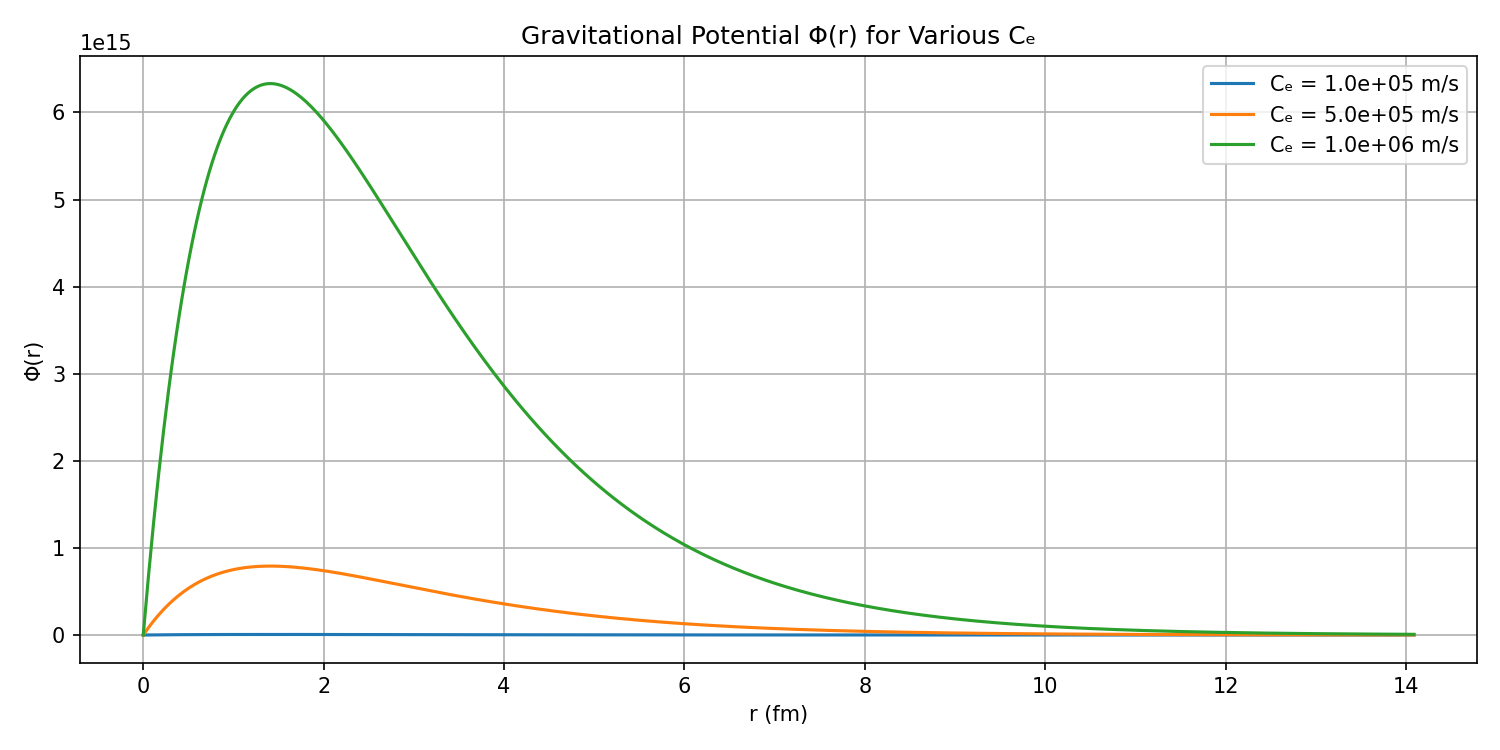
\includegraphics[width=0.8\textwidth]{images/plotG}
        \caption{Simulated gravitational potential \( \Phi(r) \) for varying \( C_e \) values.}
    \end{figure}

    \begin{figure}[h!]
        \centering
        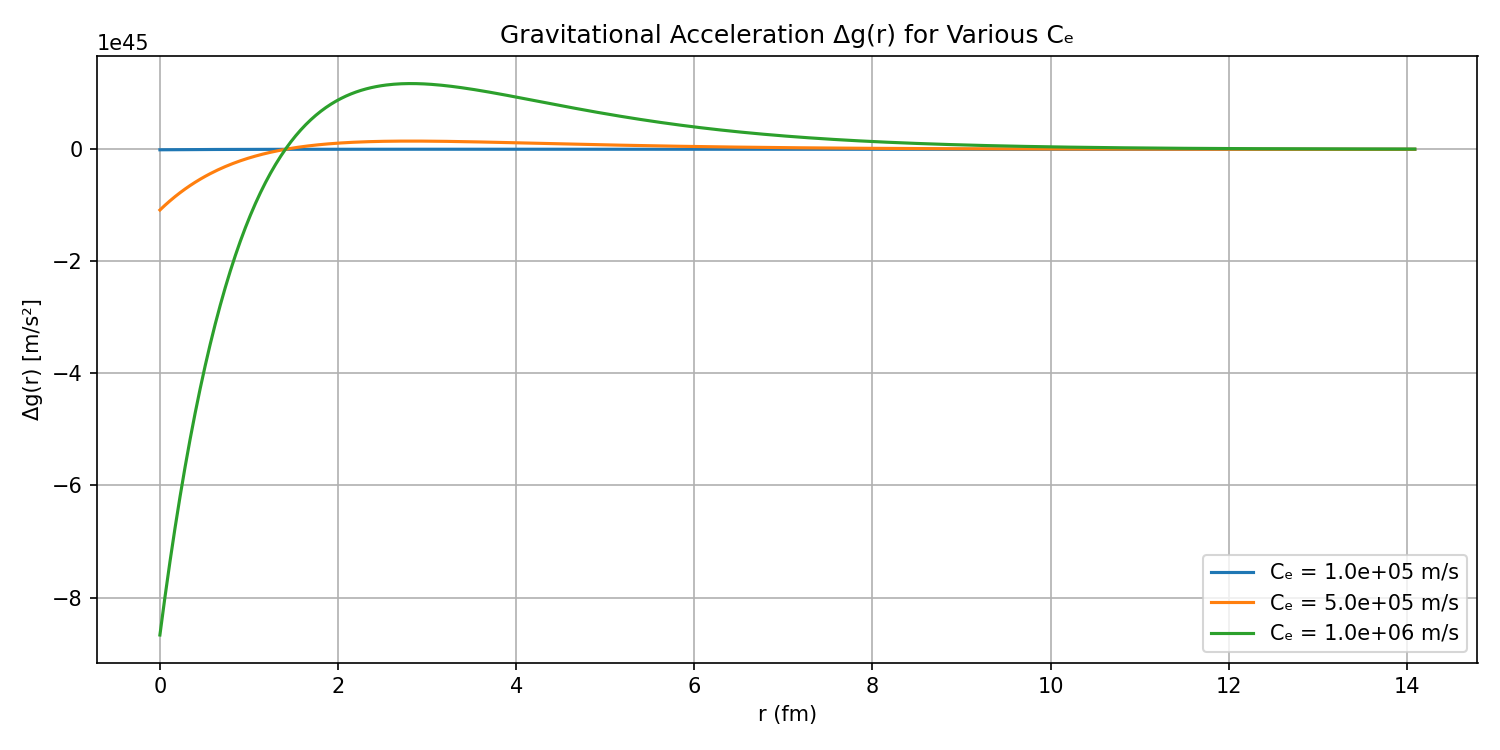
\includegraphics[width=0.8\textwidth]{images/plotG2}
        \caption{Predicted gravitational modulation \( \Delta g(r) \) across radius \( r \), showing peak amplitude shifts with \( C_e \).}
    \end{figure}

    \subsection*{Sensor Sensitivity Comparison}
    We compare the expected signal against published sensitivities:

    \begin{table}[h!]
        \centering
        \begin{tabular}{|l|c|c|}
            \hline
            \textbf{Instrument} & \textbf{Sensitivity} & \textbf{Reference} \\
            \hline
            Quantum Gravimeter & \( \sim 10^{-10} \, \si{m/s^2} \) & Menoret et al. (2018) \\
            MEMS Gravimeter & \( \sim 10^{-8} \, \si{m/s^2} \) & Hwang et al. (2021) \\
            Atom Interferometer & \( \sim 10^{-11} \, \si{m/s^2} \) & Freier et al. (2016) \\
            \hline
        \end{tabular}
        \caption{Sensitivity of current gravimetric sensors. Predicted modulation for \( C_e \sim 10^6\, \si{m/s} \) lies within measurable range.}
    \end{table}


% ============== End of content =============
%
%% === Bibliography (only for standalone) ===
%\ifdefined\standalonechapter\else
%\bibliographystyle{unsrt}
%\bibliography{../../references}
%\end{document}
%\fi